\documentclass[conference]{IEEEtran}
\IEEEoverridecommandlockouts
% T1 fontenc is required for Turkish accented letters (ğ, ş, ı, İ, ö, ü, ç)
% to compose correctly under pdflatex -- without it, OT1 has no precomposed
% glyphs for e.g. g-breve and the accent renders as a stray floating mark
% instead of attaching to its base letter.
\usepackage[T1]{fontenc}
\usepackage[utf8]{inputenc}
\usepackage{cite}
\usepackage{amsmath,amssymb,amsfonts}
\usepackage{graphicx}
\usepackage{textcomp}
\usepackage{xcolor}
\usepackage{booktabs}
\usepackage{hyperref}
% hyperref's default draws a visible colour-bordered box around every link
% target, including \cite and \ref -- hidelinks keeps them clickable in the
% PDF without the box/colour, which is what a print-ready submission wants.
\hypersetup{hidelinks}
% Use the scalable Latin Modern Typewriter face for code identifiers. This
% keeps IEEEtran's Times body face unchanged while avoiding bitmap Type 3
% glyphs in the camera-ready PDF.
\renewcommand{\ttdefault}{lmtt}

\begin{document}

\title{Cache-Aware Request Routing for Distributed RAG-Based LLM Serving:\\
Design, Calibration, and Empirical Findings}

\author{
\IEEEauthorblockN{Saadet Cansu Baktıroğlu}
\IEEEauthorblockA{Dept.\ of Artificial Intelligence \\ Engineering\\
TOBB University\\
of Economics and Technology\\
Student ID: 231401023 \\
sbaktiroglu@etu.edu.tr}
\and
\IEEEauthorblockN{Umut Baran Boztaş}
\IEEEauthorblockA{Dept.\ of Computer Engineering\\
TOBB University \\
of Economics and Technology\\
Student ID: 231101064 \\
uboztas@etu.edu.tr}
\and
\IEEEauthorblockN{Demir Doruk Dilek}
\IEEEauthorblockA{Dept.\ of Computer Engineering\\
TOBB University\\
of Economics and Technology\\
Student ID: 231104088 \\
demirdoruk.dilek@etu.edu.tr}
}

\maketitle

\begin{abstract}
Retrieval-augmented generation (RAG) over replicated large language
model (LLM) servers creates a joint decision: the router must select a
replica and order the retrieved chunks so that their prefix matches that
replica's KV cache. We implement this decision in an
OpenAI-compatible router for two vLLM workers and evaluate five core
strategies under calibrated cache capacity, cold starts, rotated arm
order, 800-request traces, and three repetitions. Cache-blind policies
reuse 55.5--56.2\% of prompt tokens, flat cache-aware policies reach
66.1--66.4\%, and the worker-specific joint strategy
\texttt{per\_worker\_tree} reaches $76.1\pm0.06\%$, a 9.7 percentage
point gain over \texttt{cache\_aware}. The gain grows to 12.0 points at
the highest replicated load and falls to 4.2 points on a low-locality
trace, consistent with the proposed cache-locality mechanism. Its
reported 10.7$\times$ median-TTFT advantage at that load is only a
completion-path measurement, however, and is not an end-to-end speedup.
Repeated controls do not separate \texttt{cache\_aware} from the local
DualMap-inspired prototype, nor fixed from overlap-adaptive routing; a
semantic-labelled arm is a protocol no-op at two workers. Recalibrating
tracker capacity preserves the earlier ordering ranking but eliminates
the previously reported beta-by-load/locality crossover. Dispatch-time
cache bookkeeping remains more rank-accurate under load than
completion-time bookkeeping. We report these negative replications,
prompt-serialization and raw-artifact limitations explicitly, and add
sweep tooling that records end-to-end timing, p99 latency, load
coefficient of variation, and file-backed router logs.
\end{abstract}

\begin{IEEEkeywords}
LLM serving, KV cache, prefix caching, request routing, retrieval-augmented generation, load balancing, vLLM
\end{IEEEkeywords}

\section{Introduction}

Serving large language models behind a pool of replicas is now standard
practice for throughput and availability. When the workload is
retrieval-augmented -- each request's prompt is built from a fixed
system preamble followed by a handful of retrieved document chunks --
the serving engine's prefix KV cache can eliminate most of the prefill
cost for a request \emph{if} it is routed to a replica that already
holds a matching prefix in cache. A router that is blind to this fact
(round robin, or load balancing on queue depth alone) discards a large,
freely available source of latency reduction: which replica currently
holds which prefix is entirely a function of routing history, so the
router itself controls the very signal it would need to route well.

This paper describes a cache-aware router built as a transparent
reverse proxy in front of $N$ vLLM~\cite{kwon2023vllm} replicas. Its
starting point is a shared scoring function,

\[
\text{score}(w) = \alpha \cdot \text{cache\_gain}(w) - \beta \cdot \text{load}(w),
\]

of which round-robin, pure load balancing, and cache-aware routing are
special cases. The central extension keeps a separate history tree for
each worker and evaluates that worker's best cache-friendly chunk order
jointly with its load, rather than computing one global order and then
routing it.

The evaluation makes four contributions:

\begin{enumerate}
  \item \textbf{Calibrated system comparison.} A five-arm, three-run
  sweep compares two cache-blind baselines, two flat cache-aware
  policies, and worker-specific joint routing/reordering. At speedup
  eight, \texttt{per\_worker\_tree} raises aggregate cached-token
  fraction from $66.4\pm0.4\%$ to $76.1\pm0.06\%$ relative to
  \texttt{cache\_aware}, while contains-gold quality remains within the
  77.5--77.8\% band.
  \item \textbf{Mechanism-oriented axes.} Repeated load and locality
  sweeps show a 9.7--12.0 point gain at the two replicated load points,
  but only 4.2 points under low locality. This conditionality is more
  informative than a single winner at one operating point.
  \item \textbf{Negative replications.} Three runs do not separate
  \texttt{cache\_aware} from \texttt{cacheweaver\_dualmap}, fixed from
  overlap-adaptive routing, or the reported semantic-labelled arm from
  its non-semantic parent. Calibrated beta sweeps do not reproduce the
  earlier crossover pattern. We treat ``not separated'' as an
  uncertainty statement, not equivalence.
  \item \textbf{Measurement controls.} The cache tracker is calibrated
  to 5{,}840 blocks; arm order is rotated; engines and router are cold
  reset; schedule lag, p99 latency, load CV, quality, decision time, and
  end-to-end timing are recorded. File-backed Uvicorn logs remove an
  unread-pipe deadlock that had been misdiagnosed as strategy overload.
\end{enumerate}

The result also requires two qualifications. First, the historical
\texttt{per\_worker\_tree} timings start after the preliminary decision
call and therefore cannot establish an end-to-end latency advantage.
Second, that two-phase run used a chunk separator adding 45 prompt
tokens per request, producing a 1.9\% denominator mismatch relative to
one-phase arms. The revised harness fixes the serialization and records
both completion-path and end-to-end timing, but the reported measurements
predate that fix. Our claim is therefore about the measured cache-fraction
separation under the stated protocol, not a protocol-neutral latency
speedup. The central question is correspondingly conditional: when does
worker-aware ordering add value, and how does that value change as load
and retrievable overlap change?

\section{Related Work}

Three largely separate literature threads intersect with this work:
distributed cache-affinity routing, RAG-specific cache reuse, and
adaptive/semantic parameter tuning. Table~\ref{tab:relatedwork}
positions the systems most relevant to the implementation;
vLLM~\cite{kwon2023vllm} underlies the serving engine and is discussed
separately at the end of this section.

\subsection{Distributed Cache-Affinity Routing}

Preble~\cite{preble2025} routes requests sharing a prefix to the same
replica to maximise KV-cache reuse, maintaining a precise prefix tree
per replica and switching from prompt-aware to load-aware scheduling
once a request's prefix-hit rate falls below a threshold.
Mooncake~\cite{mooncake2025} disaggregates prefill and decode into
separate clusters around a KVCache-centric scheduler that balances
throughput against latency SLOs. NVIDIA Dynamo~\cite{dynamo2025}
implements a production KV-cache-aware router that scores replicas on
a combined decode-cost/prefill-cost estimate derived from cache
overlap. DualMap~\cite{dualmap2026} identifies a shared weakness across
this line of work -- oscillating between a single cache-affinity
objective and a single load-balancing objective in one shared mapping
space -- and proposes a ``power of two choices''-style fix: each
request is mapped to two independent candidate replicas via two
independent hashes, with SLO-aware routing and hotspot-aware
rebalancing arbitrating between them.

This thread solves worker selection but is \emph{not RAG-specific}: it
treats the prefix as a fixed session history and does not address the
fact that retrieval returns a \emph{set} of documents whose order can
differ from one query to the next even when the set itself overlaps
heavily with a previous query's.

\subsection{RAG-Specific Cache Reuse}

RAGCache~\cite{ragcache2024} builds a knowledge tree over retrieved
document sequences and caches intermediate states across the GPU/host
memory hierarchy, additionally overlapping retrieval with speculative
generation. CacheBlend~\cite{cacheblend2025} and
TurboRAG~\cite{turborag2025} target the case where reusable chunks do
\emph{not} form a contiguous prefix at all, fusing precomputed KV
caches (selectively recomputing only a small subset of tokens to
preserve generation quality) rather than relying on prefix alignment.
Cache-Craft~\cite{cachecraft2025} shows that plain prefix caching
degrades substantially on production RAG traffic and proposes
identifying which chunk-caches remain valid, cheaply repairing the
ones that do not. CacheWeaver~\cite{cacheweaver2026} -- the mechanism
this paper's \texttt{per\_worker\_tree} strategy builds on -- takes a
different, engine-unmodified approach: a lightweight prompt-layer
method that reorders retrieved chunks into a cache-friendly sequence
via a greedy prefix-tree walk (its Algorithm~1), reported to reach
97.5\% of an oracle ordering's reusable-prefix depth.

This thread addresses RAG-specific cache reuse; CacheWeaver is the
member that specifically reorders retrieved evidence. The listed
systems assume a single serving instance and do not include distributed
worker selection.

\subsection{Adaptive Tuning and Semantic Approaches}

GORGO~\cite{gorgo2026} models per-request cost as the sum of network,
queueing, and prefill terms and tunes routing weights online via an
evolutionary strategy against a held-out tuning window; it is
network-topology-aware but not RAG-specific and requires black-box
search rather than a closed-form update. The semantic-caching family
-- GPTCache~\cite{gptcache2023}, SCALM~\cite{scalm2024}, and
MeanCache~\cite{meancache2024} -- compares query embeddings and, on a
sufficiently similar match, returns a cached \emph{answer} directly,
skipping computation entirely; this operates one layer above KV-cache
reuse or worker routing and carries a distinct risk profile (a
false-positive match returns a wrong answer outright, rather than
merely costing extra prefill).

\subsection{Positioning of This Work}

\begin{table}[h]
\caption{Related work compared along three axes}
\label{tab:relatedwork}
\centering
\resizebox{\columnwidth}{!}{%
\begin{tabular}{@{}lccc@{}}
\toprule
\textbf{System} & \textbf{Dist.\ routing} & \textbf{RAG cache reuse} & \textbf{Adaptive} \\
\midrule
Preble~\cite{preble2025} & \checkmark & $\times$ & partial (threshold) \\
Mooncake~\cite{mooncake2025} & \checkmark & $\times$ & $\times$ \\
Dynamo~\cite{dynamo2025} & \checkmark & $\times$ & $\times$ \\
DualMap~\cite{dualmap2026} & \checkmark & $\times$ & $\times$ (fixed SLO) \\
RAGCache~\cite{ragcache2024} & $\times$ & \checkmark & $\times$ \\
CacheBlend~\cite{cacheblend2025} & $\times$ & \checkmark & $\times$ \\
TurboRAG~\cite{turborag2025} & $\times$ & \checkmark & $\times$ \\
Cache-Craft~\cite{cachecraft2025} & $\times$ & \checkmark & $\times$ \\
CacheWeaver~\cite{cacheweaver2026} & $\times$ & \checkmark & $\times$ \\
GORGO~\cite{gorgo2026} & \checkmark & $\times$ & \checkmark (evolutionary) \\
Semantic caching & $\times$ & $\times$ & $\times$ \\
\textbf{This work} & \checkmark & \checkmark & \checkmark (overlap-adaptive) \\
\bottomrule
\end{tabular}%
}
\end{table}

This paper combines distributed routing (Section~III-A/B/D) with
RAG-specific reordering (Section~III-C) \emph{in one system}:
retrieval output is first reordered for cache friendliness, and that
ordering is then evaluated per-replica and optimised jointly with
worker selection, rather than as two independent stages. To our
knowledge no system in the surveyed literature addresses this
specific dependency -- whether to reorder before or after choosing a
worker changes which ordering is actually optimal, since two replicas'
caches generally disagree on what is cache-friendly (Section~III-C).
Techniques from Section~II-C above (adaptive tuning and semantic
selection) are borrowed as extended evaluation components layered on
top of this core design, not presented as this paper's primary
contribution.

RAGRoute~\cite{ragroute2026} is related in spirit but orthogonal in
target: it uses a lightweight classifier before retrieval to choose
which federated data sources to query. It does not decide which LLM
replica's KV cache is most relevant to an incoming query. Section~III-F
describes the prototype semantic pre-filter explored for that distinct
decision.

\textbf{Serving infrastructure.} vLLM~\cite{kwon2023vllm} provides the
underlying PagedAttention KV-cache engine and the OpenAI-compatible API
surface this router proxies. All prefix-cache accounting in this work
is calibrated against vLLM's own reported counters
(\texttt{prompt\_tokens\_details.cached\_tokens} and the Prometheus
\texttt{vllm:prefix\_cache\_*} series) rather than assumed.

\section{System Design}

\subsection{Architecture}

The router is a FastAPI reverse proxy exposing the same
\texttt{/v1/chat/completions}, \texttt{/v1/completions}, and
\texttt{/v1/models} surface as vLLM itself, so that a client (in our
deployment, an Open WebUI instance) cannot distinguish it from talking
to a bare engine -- streaming responses are forwarded byte-for-byte
rather than buffered. A background poller scrapes each worker's
\texttt{/metrics} endpoint on a fixed interval and maintains a
per-worker \texttt{WorkerState} snapshot (queue depth, running-request
count, KV-cache utilisation, prefix-cache hit counters); routing
decisions read this snapshot rather than querying workers synchronously
on the request path.

Because vLLM exposes aggregate cache statistics but not "do you
currently hold a cache entry for this specific prefix", the router
keeps its own approximation: for each worker, an LRU of block-aligned
prefix hashes it has been sent (\texttt{PrefixTracker}), hashed in the
same fixed token-block granularity vLLM itself uses. Two independent
bookkeeping conventions are supported for \emph{when} a block is
recorded as cached -- at dispatch time (optimistic: the block will be
resident once prefill starts) or at completion time (conservative: only
once the engine has actually finished) -- and Section~VI-F reports the
result of ablating between them.

\begin{figure}[t]
\centering
\fbox{\begin{minipage}{0.92\columnwidth}
\centering\small
Client/retriever: query + unordered chunk ids\\
$\downarrow$ \texttt{/router/decide\_order}\\
Router: choose worker + worker-specific order\\
$\downarrow$ returned worker and ordered ids\\
Client: assemble the ordered prompt\\
$\downarrow$ forced completion request\\
Selected vLLM worker
\end{minipage}}
\caption{Current client-mediated two-phase path. The client applies the
returned order. The revised replay harness records decision,
completion-path, and end-to-end timings separately; the historical
results in Section~VI used only the completion-path timer.}
\label{fig:two-phase}
\end{figure}

\subsection{Strategy Framework}

All registered strategies share a common interface,
\texttt{select(context, snapshot) -> Decision}, so that switching the
active policy is a configuration change rather than a code change. Five
policies use the ordinary one-phase proxy path:

\begin{itemize}
  \item \textbf{round\_robin}: $\alpha{=}\beta{=}0$, plus a rotating
  tie-break; the floor every other strategy is measured against.
  \item \textbf{least\_loaded}: $\alpha{=}0$; pure, cache-blind load
  balancing on a saturating load-normalisation
  $\text{load\_norm}(w) = \text{load}(w) / (\text{load}(w) +
  \text{LOAD\_REF})$, chosen over a clipped $\min(\cdot,1)$ form because
  clipping destroys the policy's discriminative power once both
  replicas exceed the reference load (Section~IV-C).
  \item \textbf{cache\_aware}: the full scoring function plus an
  \emph{adaptive guard band}, $\delta = \delta_0 \cdot (1 -
  \overline{\text{kv\_usage}})$: the winning replica by score is
  overridden back to the least-loaded replica if its load exceeds the
  minimum by more than $\delta$. This prevents the classic failure
  mode of pure cache-affinity routing, where the replica holding a
  popular prefix keeps attracting traffic until its queue makes it the
  worst choice by latency despite remaining the best choice by cache.
  \item \textbf{adaptive\_cache\_aware}: \texttt{cache\_aware} with
  $\beta$ and $\delta_0$ driven by an overlap EWMA, while a CUSUM
  detector records diagnostic drift alarms (Section~III-E).
  \item \textbf{cacheweaver\_dualmap}: the DualMap-inspired two-choice
  prototype
  described in Section~III-D.
\end{itemize}

The two remaining registry entries, \texttt{per\_worker\_tree} and
\texttt{semantic\_per\_worker\_tree}, expose the separate decision
capability described next. This registry taxonomy must not be confused
with the arms of any one experiment: Section~VI-A compares complete
system strategies, while Section~VI-D isolates order under fixed
routing.

\subsection{Worker-Specific Joint Reordering (\texttt{per\_worker\_tree})}

DualMap's replica candidate-selection step (its Eq.~5) hashes the
reordered chunk sequence through two independent consistent-hashing
rings to obtain a candidate pair $(r_1, r_2)$, with a collision rule
$r_2 \leftarrow (r_1+1) \bmod n$ when the two rings agree. At $n{=}2$
replicas -- the deployment size used throughout this work -- this
collision rule is not an edge case: it is provably always triggered or
already trivially satisfied, so $\{r_1, r_2\} = \{0, 1\}$ on every
request. The dual-hash candidate-selection machinery is therefore a
mathematically guaranteed no-op at this scale, and any cache-affinity
signal has to come from elsewhere in the pipeline.

\texttt{per\_worker\_tree} replaces the hash-and-select step entirely.
Each worker maintains its own independent CacheWeaver knowledge tree;
for every candidate worker, \texttt{best\_reorder\_for()} computes both
that worker's own best reordering of the retrieved chunks \emph{and} a
normalised cache-gain figure against that specific tree, and the
scoring function from Section~III-B picks the winner directly -- there
is no candidate-pruning step to degenerate. This is a genuine change in
what "the right chunk order" means: it is no longer a single,
worker-independent quantity computed once and then assigned to
whichever replica is chosen, but something that emerges jointly with
the worker decision, since the two replicas' trees generally disagree
about which order is cache-friendly.

Because the winner and its optimal chunk order are decided together, a
client-mediated two-step protocol is used (Fig.~\ref{fig:two-phase}).
The client first calls
\texttt{/router/decide\_order} with the unordered, retrieval-order
chunk ids and receives back \{worker, ordered\_chunk\_ids\}; it then
builds the prompt in that returned order and issues the completion with
an \texttt{x-router-force-worker} header. The router forwards this
already ordered prompt to the named worker. Phase-one bookkeeping is
optimistic: the tree is updated before phase two succeeds, so the two
HTTP calls are not transactional.

\subsubsection{Token-weighted cache gain} The router module has an
optional token-weighted path,
$\text{gain}=\text{hit\_tokens}/\text{total\_tokens}$, for cases where
the caller supplies a chunk-id-to-text mapping. It reuses the existing
tokenizer and a synthetic regression test confirms that few large
chunks and many small chunks can select different workers. This path is
\emph{not live-integrated}: \texttt{/router/decide\_order} currently
accepts only chunk ids, and the strategy calls the module without chunk
texts. Consequently each chunk has weight one on the live HTTP path and
all reported live \texttt{per\_worker\_tree} traffic remains
chunk-count-based. Section~VI-G is therefore an isolated functional
test, not a measured live improvement.

\subsubsection{Quality protection (\texttt{protect\_top\_k})} Pure
greedy reordering can push a highly relevant but uncached chunk to the
end of the prompt while pulling a barely relevant but cached chunk to
the front -- a risk CacheWeaver's own evaluation does not fully rule
out (its Table~7 states only that reordering \emph{did not measurably
hurt} answer quality in their setting, not that it never can).
\texttt{protect\_top\_k} pins the first $K$ retrieval-order chunks in
the returned list and reorders only what follows; $K{=}0$ reproduces the
original behaviour. A regression test verifies this positional
property. It does not establish that the post-pinned traversal remains
one cache-contiguous prefix when a pinned chunk is absent from the
tree, nor does it establish answer quality; both require end-to-end
validation.

\subsection{The \texttt{cacheweaver\_dualmap} Baseline and a Tie-Break Defect}

DualMap's official implementation (\url{https://github.com/ASISys/DualMap},
MIT-licensed, which also incorporates Preble) is publicly available,
but was not used directly: it is written against an 8+-GPU, 512\,GB-DRAM
reference deployment and consumes Mooncake-format traces (fixed
prefixes, no real retrieval step), neither of which matches this
project's two-machine RAG deployment with genuine per-query retrieval.
The local \texttt{cacheweaver\_dualmap} strategy is therefore a
\emph{DualMap-inspired two-choice prototype}, not an equivalent
reimplementation. It uses two independent BLAKE2b-modulo mappings
rather than consistent-hash rings, estimates recompute cost with a
fixed 200-token-per-chunk placeholder, and derives pending-token load
from vLLM's waiting-request gauge. On the documented vLLM V1 setup that
gauge can remain zero under load, so SLO/rebalancing activation has not
been demonstrated. Moreover, although the inner prototype computes a
CacheWeaver order, the enclosing strategy does not propagate that order
to the proxy's prompt-rewrite field; vLLM therefore receives the
original prompt order in the reported one-phase runs. Results bearing
this strategy name evaluate its current two-choice routing and internal
bookkeeping, not live CacheWeaver reordering or a faithful DualMap run.

An earlier internal version also used one shared tree for both
replicas, making their recompute estimates identical. Per-replica trees
fixed that error but exposed a separate tie defect: non-strict
comparisons always selected the hash-assigned $r_1$ when estimates tied.
The current implementation randomises this candidate tie; Section~VI-G
describes the corresponding GPU-free regression test.

\subsection{Overlap-Adaptive Weighting}

A common formula underlies the adaptive modes: Jaccard overlap
$J(A,B)=|A\cap B|/|A\cup B|$. The current call sites do \emph{not},
however, observe the same stream. \texttt{adaptive\_cache\_aware}
compares adjacent requests within each session, whereas
\texttt{per\_worker\_tree}'s modes compare globally adjacent requests
and initialise the first comparison against an empty set. The offline
tool reports both notions separately (Section~IV-D); sharing a formula
does not make their calibrated values interchangeable.

\textbf{Threshold mode.} A one-line switch: $\alpha{=}0.2,\ \beta{=}0.8$
when $J$ falls below a configured threshold (locality is a weak
signal, weight load instead), and $\alpha{=}0.8,\ \beta{=}0.2$
otherwise, with $\alpha+\beta{=}1$ by construction.

\textbf{EWMA with CUSUM diagnostics.} An exponentially weighted moving average
tracks a smoothed overlap estimate $D_t = \lambda J_t + (1-\lambda)
D_{t-1}$. This EWMA, together with the fixed configured
$D_{\text{target}}$, feeds
$\beta_{\text{live}} = \beta_{\text{base}} \cdot \text{clip}\!\left(1 +
k\cdot\frac{D_{\text{target}} - D_t}{D_{\text{target}}},\,
[0.3, 3.0]\right)$, while $\alpha$ is held fixed. A CUSUM detector is
updated alongside it and recalibrates its own alarm reference, but the
returned alarm and recalibrated reference are not consumed by routing.
CUSUM is therefore observational telemetry in the current code, not a
second decision input. Offline calibration now reconstructs the exact
arrival-ordered, within-session stream observed by
\texttt{adaptive\_cache\_aware}; at retrieval depth ten this gives
\texttt{D\_TARGET=0.322} and favours \texttt{CUSUM\_H=0.30} over the
previous 0.20 default. The per-worker mode still consumes global
adjacency, so the calibrated target is not transferable to that path.
GPU-free tests verify that \texttt{off} reproduces the fixed baseline
and that threshold/EWMA inputs can change a synthetic decision. The
live hot and drifted comparisons in Section~VI-C find no outcome
separation at three repetitions.

\subsection{Semantic Candidate Pre-Filtering}

For deployments with more than a handful of replicas,
\texttt{per\_worker\_tree}'s $O(k^2)$ per-candidate reorder becomes
$n \cdot O(k^2)$ across all healthy workers -- cheap at $n{=}2$, not
necessarily cheap beyond it. \texttt{SemanticWorkerRouter} addresses
this independently of locality-based weighting: each worker's recent
query traffic is summarised as an EWMA centroid in embedding space
(\texttt{multilingual-e5-base}, the same checkpoint used for corpus
retrieval, loaded once per router process); an incoming
query is embedded and ranked by cosine similarity against each
worker's centroid, and only the top-$k$ ranked workers are passed to
\texttt{per\_worker\_tree}'s comparison. A worker with no observed
traffic yet is assigned the \emph{average} similarity of workers that
do have a centroid -- neither a fixed low score (which would
permanently exclude new or recently restarted workers) nor a fixed
high score (which would make every cold worker an automatic favourite)
-- and the candidate set falls back to every healthy worker whenever
the semantic favourites happen to be unhealthy, so the mechanism cannot
starve a request. Loading the embedding model is forced synchronously
at router start-up rather than being paid by whichever live request
happens to arrive first.

The reported semantic-labelled arm cannot exercise the intended
pre-filter: \texttt{SEMANTIC\_TOP\_K=2} equals the entire two-worker
pool, so no candidate is removed. The revised two-phase contract now
carries query text and the experiment runner can request top-$k{=}1$;
those changes make a future active ablation possible but do not
retroactively turn the reported no-op into a semantic result. A
scalable evaluation still requires $N>k$ and must include embedding
overhead in end-to-end timing.

\section{Implementation Details}

\subsection{Corpus and Trace Construction}

The RAG corpus is built from the publicly available TQuAD
dataset~\cite{tquad}, a SQuAD-format Turkish question-answering resource
(681 articles, 8{,}308 questions). Each
question already points at exactly one source paragraph, so using the
paragraph as the retrieval chunk gives retrieval ground truth "for
free". Paragraphs are split at sentence boundaries only when they
exceed a maximum chunk length, and every chunk is padded (in token
space, not by appending raw text -- tokenizers merge whitespace
unpredictably) to a multiple of vLLM's KV-cache block size, since a
chunk boundary that does not align with a block boundary produces a
different block hash even when the underlying content is shared,
silently breaking the prefix chain the whole system depends on. The
resulting corpus contains 2{,}619 chunks. Before padding, lengths range
from 9 to 754 tokens (mean 182.2, $\sigma{=}108.5$); after padding they
range from 16 to 768 tokens (mean 189.6, $\sigma{=}108.4$). The
variation motivates the token-weighted prototype of Section~III-C.1,
but that prototype is not yet connected to live requests.

Synthetic request traces are generated once per experiment and replayed
identically across every strategy under comparison, so that strategies
are never compared against different workloads. Two independent knobs
control cache locality: popularity skew across titles (a Zipf
distribution with configurable exponent $s$) decides \emph{which}
chunks are asked about repeatedly, and session structure (several
questions drawn from one title, arriving with realistic think-time
gaps) decides \emph{when} repeats occur relative to each other -- a
popular chunk asked about ten times over an hour is not locality if the
cache empties between hits. An optional popularity-drift knob rotates
the ranking over the course of a trace, exercising the scenario an
adaptive policy is meant to handle and a static one is meant to
degrade gracefully under.

\subsection{Software and Deployment Platform}

The implementation is written in Python and uses FastAPI and Uvicorn for
the OpenAI-compatible reverse proxy, \texttt{httpx} for asynchronous
stream forwarding and worker polling, and \texttt{prometheus-client}
for router instrumentation. Each upstream runs vLLM with
Qwen2.5-7B-Instruct; the two workers communicate with the router over a
private Tailscale network. Hugging Face Transformers supplies the
serving-model tokenizer, \texttt{multilingual-e5-base} supplies corpus
and query embeddings, and NumPy stores and scores the offline embedding
matrix. The submission also contains replay, trace-generation,
calibration, quality-scoring, schedule-lag, and GPU-free regression
scripts. Runtime parameters, worker addresses, strategy selection, and
calibration constants are exposed as environment variables rather than
requiring source edits.

\subsection{Calibration Discipline}

\begin{table}[h]
\caption{Calibrated settings and documented experimental exceptions}
\label{tab:calibration}
\centering
\begin{tabular}{@{}p{0.29\linewidth}p{0.22\linewidth}p{0.37\linewidth}@{}}
\toprule
\textbf{Constant} & \textbf{Value} & \textbf{Measured via} \\
\midrule
\texttt{LOAD\_REF} & 16 concurrent requests & Kleinrock power (throughput/latency) peak, single-worker concurrency sweep, Qwen2.5-7B, $\sim$1700-token prompts \\
Mean prompt size & 2{,}392 tokens & Mean prompt token count, $n{=}800$ live RAG requests, top-$k{=}10$ \\
DualMap-inspired SLO / rebalance thresholds & 38{,}272 / 57{,}408 tokens & \texttt{LOAD\_REF} $\times$ mean prompt tokens; 1.5$\times$ ratio preserved from DualMap's relationship \\
\texttt{D\_TARGET} (drift reference) & 0.322 & Arrival-ordered within-session Jaccard stream, top-$k{=}10$, 2{,}170 stable observations \\
\texttt{CUSUM\_H} & 0.30 & Grid calibration on nominal and drift-0.1 traces; 26.73 nominal alarms/1{,}000 and 2.20$\times$ separation \\
\texttt{TRACKER\_CAPACITY} & 5{,}840 blocks & Smaller worker's KV-cache capacity: $\min(93{,}440,93{,}840)/16$ \\
\bottomrule
\end{tabular}
\end{table}

Table~\ref{tab:calibration} records the values used by the main strategy,
load/locality, calibrated-ordering, and calibrated-beta experiments.
Semantic top-$k$, centroid learning rate,
CUSUM margin $K$, EWMA rate, and \texttt{protect\_top\_k} retain explicit
prototype defaults. The source default for \texttt{TRACKER\_CAPACITY}
is 50{,}000; calibrated routing experiments require
\texttt{ROUTER\_TRACKER\_CAPACITY=5840}. Only the historical
dispatch/completion sweep and the original ordering run used 50{,}000;
both held it fixed across arms and are labelled as historical
exceptions. Section~VI-D reports the ordering replication at 5{,}840.

\subsection{Overlap Characterisation Tool}

A standalone tool computes the Jaccard overlap between consecutive
requests' retrieved chunk sets directly from a corpus and trace,
without touching the router or a live engine (retrieval alone is
enough). It reports two distinct notions of "consecutive" separately,
because they answer different questions: \emph{session-adjacent}
overlap (turn $k$ to turn $k{+}1$ within one session) reflects what a
prefix cache actually sees if the router keeps a session pinned to one
worker, while \emph{global-adjacent} overlap (arrival-order adjacency,
ignoring session boundaries) reflects the raw opportunity the router
faces before any session-affinity policy is applied. This distinction
turns out to matter a great deal (Section~VI-G).

\section{Experimental Setup}

All live experiments use two RTX~4090 workers running
Qwen2.5-7B-Instruct with GPU-memory utilisation 0.85; one is local and
the other is reached over Tailscale. Requests are released at their
trace offsets without waiting for earlier completions. Before each arm,
both engines and the router are restarted to clear their cache and
tracker state. Arms are interleaved repeat-major and rotated across
repetitions. The router's estimated cached tokens are checked against
vLLM's \texttt{prompt\_tokens\_details.cached\_tokens} response field.

\begin{table}[t]
\caption{Experiment families and protocol scope}
\label{tab:protocol}
\centering
\footnotesize
\setlength{\tabcolsep}{3pt}
\begin{tabular}{@{}p{0.28\linewidth}p{0.62\linewidth}@{}}
\toprule
\textbf{Family} & \textbf{Protocol} \\
\midrule
Core strategies & 800 requests, top-$k{=}10$, speedup 8, five arms,
three repetitions, capacity 5{,}840 \\
Load/locality & \texttt{cache\_aware} vs. \texttt{per\_worker\_tree};
speedups 4/8/12 and high/low synthetic locality \\
Adaptive/semantic & Three repetitions on hot and drift-0.1 traces;
semantic arm retains all two candidates \\
Ordering & Four fixed-router orders, top-$k{=}10$, three repetitions;
original 50{,}000 and calibrated 5{,}840 capacities \\
Beta & High/low locality $\times$ speedups 30/35 $\times\beta\in\{0,1\}$;
one retained result per cell at capacity 5{,}840 \\
Bookkeeping & Dispatch vs. completion, speedups 5/15, three repetitions;
historical capacity 50{,}000 \\
\bottomrule
\end{tabular}
\end{table}

The high-locality trace uses Zipf $s{=}1.5$ and session length four;
the low-locality trace uses $s{=}0.7$ and session length two. The main
15 runs have schedule-lag p99 at most 2\,ms. At the selected operating
point, tracker validation gives Pearson correlation 1.000, mean
absolute error 0.6 token, and zero underestimation. Speedup eight avoids
both the weak top-$k{=}3$, speedup-five regime, where strategies cluster,
and speedup 20, where median TTFT reaches 8.8\,s and queueing dominates.

For each run, cache reuse is $\sum$ cached prompt tokens divided by
$\sum$ prompt tokens. We report TTFT p50 and p99, request-count load CV
including zero-count workers, and normalised output ``contains gold''
as the primary quality check. Means use the sample standard deviation
over repetitions. As a descriptive separation rule, a mean difference
must exceed twice the larger arm standard deviation; failing that rule
means unresolved, not equivalent. The historical ordering scorer uses
the mean of per-request cache fractions instead of the run-level
aggregate and is labelled separately.

The reported two-phase \texttt{per\_worker\_tree} runs time only the
completion request. Their decision call, prompt construction, and first
HTTP round trip are excluded. They also use a separator five tokens
longer at each of nine boundaries, adding about 36{,}000 prompt tokens
over 800 requests (35{,}997 observed, 1.9\%). The revised replay code
uses matched serialization and records decision, completion, and
end-to-end fields, but the historical numerical results were not rerun
after that fix.

\section{Results}

\textbf{Artifact status.} The repository includes the overlap scores,
trace manifests, experiment drivers, calibration tools, regression
tests, and a configuration-recording sweep harness. It does not retain
the raw live-run JSONL outputs underlying the numerical live tables.
Those values are preserved in the project log and final report but
cannot be recomputed from the submitted tree without rerunning the two
vLLM workers.

\subsection{Calibrated Core Strategy Comparison}

\begin{table*}[t]
\caption{Calibrated five-strategy comparison at speedup 8 (mean $\pm$
sample standard deviation, three runs; cache is aggregate cached/prompt
tokens).}
\label{tab:core}
\centering
\small
\begin{tabular}{@{}lccccc@{}}
\toprule
\textbf{Strategy} & \textbf{Cached fraction} & \textbf{TTFT p50} &
\textbf{TTFT p99} & \textbf{Load CV} & \textbf{Contains gold} \\
\midrule
\texttt{least\_loaded} & $55.5{\pm}0.8\%$ & $0.785{\pm}0.126$\,s & $3.368{\pm}0.739$\,s & 0.008 & $77.8{\pm}0.3\%$ \\
\texttt{round\_robin} & $56.2{\pm}0.2\%$ & $0.742{\pm}0.063$\,s & $2.564{\pm}0.082$\,s & 0.000 & $77.7{\pm}0.3\%$ \\
\texttt{cacheweaver\_dualmap} & $66.1{\pm}0.6\%$ & $0.484{\pm}0.303$\,s & $2.633{\pm}0.679$\,s & 0.358 & $77.7{\pm}0.1\%$ \\
\texttt{cache\_aware} & $66.4{\pm}0.4\%$ & $0.278{\pm}0.028$\,s & $2.320{\pm}0.645$\,s & 0.260 & $77.5{\pm}0.1\%$ \\
\textbf{\texttt{per\_worker\_tree}} & $\mathbf{76.1{\pm}0.06\%}$ & $0.147{\pm}0.001$\,s$^\dagger$ & $1.184{\pm}0.190$\,s$^\dagger$ & 0.196 & $77.6{\pm}0.15\%$ \\
\bottomrule
\end{tabular}
\par\vspace{2pt}
{\footnotesize $^\dagger$ Completion-path timing; the decision call and first
HTTP round trip are excluded.\par}
\end{table*}

Table~\ref{tab:core} supplies the paper's previously missing system-level
comparison. Flat cache-aware routing adds 10.9 points over
\texttt{least\_loaded}; worker-specific joint routing and ordering adds
another 9.7 points over \texttt{cache\_aware}. Both clear the descriptive
spread threshold (1.6 and 0.9 points, respectively). The five quality
means occupy a narrow 77.5--77.8\% band. Conversely,
\texttt{cache\_aware} and \texttt{cacheweaver\_dualmap} do not separate
on cache reuse, p50, or p99; the earlier single-run latency difference
was noise at this replication level. The \texttt{per\_worker\_tree}
p99 gap also narrowly fails the spread rule, and its p50/p99 values must
not be read as end-to-end comparisons because of the two-phase timer.

\subsection{Load and Locality Characterisation}

\begin{figure*}[t]
\centering
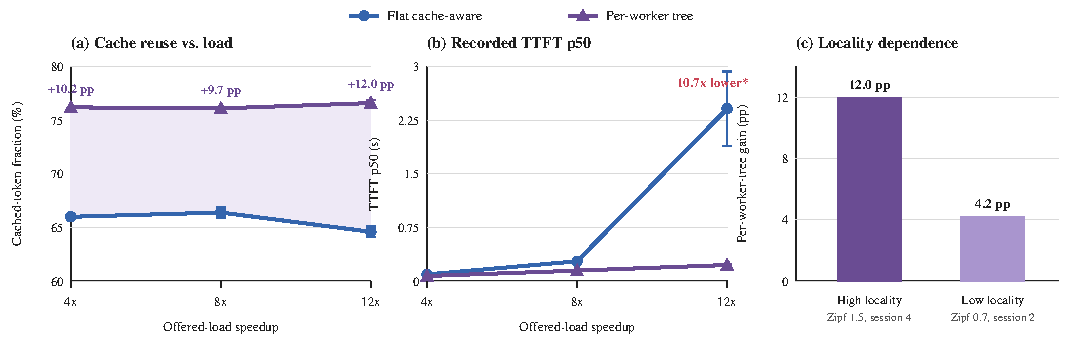
\includegraphics[width=\textwidth]{figures/result_summary.pdf}
\caption{Worker-specific routing across load and locality. At replicated
speedups 8 and 12, \texttt{per\_worker\_tree} improves cached-token
fraction over \texttt{cache\_aware} by 9.7 and 12.0 percentage points;
the 4$\times$ point has $n{=}1$ and is exploratory. Reported
\texttt{per\_worker\_tree} TTFT is completion-path timing, not end to
end. Its historical prompt separator also adds 35{,}997 prompt tokens
(1.9\%) over 800 requests, so cache denominators are not perfectly
matched.}
\label{fig:load-locality}
\end{figure*}

Figure~\ref{fig:load-locality} shows that the cache advantage remains
9.7--12.0 points at the replicated 8$\times$ and 12$\times$ loads. At
12$\times$, median completion-path TTFT is 0.226\,s versus 2.411\,s for
the one-phase baseline, a 10.7$\times$ ratio that is consistent with
less prefill work preventing queue growth but is not an end-to-end
speedup or a causal decomposition. The 4$\times$ direction is similar
(+10.2 points) but has only one run.

Locality provides the sharper mechanism check. On the high-locality
trace at speedup 12, the cache fractions are $76.6{\pm}0.3\%$ and
$64.6{\pm}0.5\%$; on the low-locality trace they fall to
$57.3{\pm}0.3\%$ and $53.1{\pm}0.1\%$. The gain therefore contracts
from 12.0 to 4.2 points, as a cache-reuse mechanism predicts. Low-locality
p99 is unresolved. Its 1.2-point contains-gold difference is directionally
consistent across runs but is not claimed as a quality improvement
without a paired question-level test.

\subsection{Repeated Null Results}

\begin{table}[t]
\caption{Replicated controls (cached-token fraction)}
\label{tab:nulls}
\centering
\footnotesize
\begin{tabular}{@{}lcc@{}}
\toprule
\textbf{Comparison} & \textbf{Arm A} & \textbf{Arm B} \\
\midrule
Adaptive / fixed, hot & $66.5{\pm}0.5\%$ & $66.4{\pm}0.5\%$ \\
Adaptive / fixed, drift 0.1 & $43.8{\pm}0.7\%$ & $44.0{\pm}0.5\%$ \\
Semantic-labelled / PWT, hot & $76.1{\pm}0.40\%$ & $76.1{\pm}0.06\%$ \\
\bottomrule
\end{tabular}
\end{table}

The adaptive policy's $\beta$ is active (405 distinct values spanning
0.65--1.28), yet neither the hot nor drifted trace separates from fixed
\texttt{cache\_aware}. CUSUM cannot explain this null result because its
alarms are telemetry and are not consumed by the router. The reported
semantic arm is a structural no-op: top-$k{=}2$ retains both workers, so
its identical hit rate says nothing about semantic usefulness. The
revised query-carrying protocol and top-$k{=}1$ option require a fresh
measurement.

\subsection{Ordering Result Survives Capacity Calibration}

\begin{table}[t]
\caption{Worker-blind ordering at original and calibrated capacities}
\label{tab:ordering}
\centering
\footnotesize
\begin{tabular}{@{}lccc@{}}
\toprule
\textbf{Order} & \textbf{50{,}000 blocks} & \textbf{5{,}840 blocks} & \textbf{Change} \\
\midrule
Greedy & $73.1{\pm}0.2\%$ & $73.2{\pm}0.3\%$ & +0.1 pp \\
Relevance & $67.7{\pm}0.1\%$ & $67.6{\pm}0.4\%$ & $-0.1$ pp \\
Canonical & $65.0{\pm}0.5\%$ & $64.9{\pm}0.2\%$ & $-0.1$ pp \\
\texttt{pinned\_prefix} & $62.9{\pm}0.2\%$ & $62.7{\pm}0.4\%$ & $-0.2$ pp \\
\bottomrule
\end{tabular}
\end{table}

This ablation holds \texttt{cache\_aware} routing fixed and changes
only one global, worker-blind prompt order. Calibration moves every mean
by at most 0.2 points and preserves the ranking: greedy is 5.6 points
above relevance and 8.3 above canonical at 5{,}840 blocks. Thus a rule
that observes estimated cache state wins; canonical and session-prefix
ordering do not. At top-$k{=}3$, a single preliminary run spans only 2.4
points, so the lever opens with retrieval depth. The result uses the
historical request-macro metric and must not be numerically conflated
with Table~\ref{tab:core}'s run-level aggregate.

\subsection{Calibrated Beta Matrix}

\begin{table}[t]
\caption{TTFT p50 in the calibrated beta matrix}
\label{tab:beta}
\centering
\footnotesize
\begin{tabular}{@{}llccc@{}}
\toprule
\textbf{Locality} & \textbf{Load} & $\boldsymbol{\beta=1}$ & $\boldsymbol{\beta=0}$ & \textbf{Direction} \\
\midrule
High & 30$\times$ & 0.175\,s & 0.484\,s & $\beta{=}1$ \\
High & 35$\times$ & 1.323\,s & 2.734\,s & $\beta{=}1$ \\
Low & 30$\times$ & 0.151\,s & 0.147\,s & unresolved \\
Low & 35$\times$ & 0.442\,s & 0.940\,s & $\beta{=}1$ \\
\bottomrule
\end{tabular}
\end{table}

Here $\beta{=}1$ includes the load term and $\beta{=}0$ is pure cache
routing. The earlier uncalibrated crossover pattern does not replicate:
$\beta{=}1$ is lower in three cells and the remaining difference is
4\,ms. Because per-cell spreads are absent from the supplied result
bundle, Table~\ref{tab:beta} reports directions rather than three
significant wins. Cache fraction is nearly unchanged across beta; the
observed differences lie in queueing behaviour.

\subsection{Bookkeeping and Drift Diagnostics}

\begin{table}[t]
\caption{Cache-state accuracy at two replay loads (three runs per mode)}
\label{tab:timing}
\centering
\footnotesize
\setlength{\tabcolsep}{2pt}
\begin{tabular}{@{}llccc@{}}
\toprule
\textbf{Spd.} & \textbf{Mode} & \textbf{Corr.} & \textbf{Rank agree.} & \textbf{Underest.} \\
\midrule
$5\times$ & Dispatch & $0.972{\pm}0.010$ & $97.1{\pm}0.6\%$ & $0.0{\pm}0.0\%$ \\
$5\times$ & Completion & $0.941{\pm}0.011$ & $92.5{\pm}0.6\%$ & $6.2{\pm}0.7\%$ \\
$15\times$ & Dispatch & $0.980{\pm}0.003$ & $98.0{\pm}0.0\%$ & $0.0{\pm}0.0\%$ \\
$15\times$ & Completion & $0.806{\pm}0.008$ & $79.7{\pm}0.9\%$ & $29.6{\pm}0.8\%$ \\
\bottomrule
\end{tabular}
\end{table}

Completion-time bookkeeping misses related requests that are still in
flight; as load rises, its correlation falls from 0.941 to 0.806 and
underestimation rises from 6.2\% to 29.6\%, while dispatch remains near
0.98 correlation. Since this historical sweep uses 50{,}000 blocks, it
supports the relative load mechanism, not calibrated absolute error.

Trace calibration changes \texttt{D\_TARGET} from 0.529 to 0.322 and
\texttt{CUSUM\_H} from 0.20 to 0.30. The latter reduces nominal alarms
from 108.76 to 26.73 per 1{,}000 and improves drift/nominal separation
from 1.52$\times$ to 2.20$\times$. A nominal trace has no labelled change
points, however, and CUSUM alarms do not affect routing; this remains
diagnostic telemetry.

\subsection{Harness Corrections and Isolated Checks}

The sweep launcher previously left Uvicorn stdout/stderr connected to
an unread pipe. Its 64-KB buffer eventually filled and blocked the
router, so the old ``two-phase overload'' diagnosis is withdrawn. Each
run now writes router output to its own log file. The shared scorer now
uses aggregate prompt-token weighting, inclusive p99, and load CV over
all expected workers; the replay records decision and end-to-end fields
and uses one separator across one- and two-phase paths.

A randomized tie replaces the DualMap-inspired arm's deterministic
first-candidate choice; a 400-request GPU-free test checks that neither
worker falls below 35\%. A separate synthetic test shows why optional
token weighting matters: two cached chunks totalling about 1{,}300
tokens should beat three cached chunks totalling about nine tokens,
although the live decision endpoint still lacks chunk texts. Finally,
offline overlap remains strongly session-structured: on the baseline
3{,}000-request trace, mean session-adjacent Jaccard is 0.476 versus
0.055 for global adjacency. These checks explain design choices but are
not additional live performance claims.

\section{Discussion and Limitations}

The combined evidence supports a mechanism-oriented conclusion.
Worker-specific joint routing/reordering adds substantial cache reuse on
the high-locality workload, the gap increases at the heavier replicated
load, and it contracts when locality is removed. This is stronger than a
single-point winner but not a universal claim. The worker-blind ordering
ablation separately shows that only cache-informed greedy ordering beats
relevance order; merely imposing canonical or session-prefix order is
harmful. Negative replications are equally informative: flat
cache-aware variants are unresolved, overlap adaptation does not change
outcomes even under drift, and beta's old crossover was not robust to
capacity calibration.

The principal threats to validity are:

\begin{enumerate}
  \item \textbf{Protocol comparability.} Historical
  \texttt{per\_worker\_tree} TTFT excludes decision/reordering and cannot
  support an end-to-end speedup claim. Its prompt contains 1.9\% more
  tokens because of a separator mismatch. The fixed harness must be
  rerun before comparing latency or exact cache fractions without this
  qualification.
  \item \textbf{Two workers and a partial baseline.} At $N{=}2$, both
  hash candidates cover the whole pool. The local DualMap-inspired
  strategy also differs from the published system in mapping,
  migration, cost estimation, and load instrumentation. It must not be
  interpreted as official DualMap. Semantic pruning also cannot be
  evaluated when $k=N$.
  \item \textbf{Synthetic, narrow workloads.} Every live trace is
  generated over the real TQuAD corpus, not captured production traffic.
  The locality axis has only two synthetic regimes, the main sweep one
  model and two GPUs, and the 4$\times$ point only one repetition.
  Generalisation requires an external trace such as ShareGPT or LMSYS.
  \item \textbf{Metric and capacity history.} The original ordering and
  bookkeeping runs use 50{,}000 blocks; only ordering was replicated at
  5{,}840. The ordering cache score is a per-request macro-average, while
  the system table aggregates tokens. Cross-table numerical comparisons
  must respect that distinction.
  \item \textbf{Run reproducibility.} The repository lacks raw live
  JSONL outputs and a complete hardware/driver manifest. The new sweep
  scripts record configuration, arm order, lag, logs, and summary files,
  but the supplied numerical tables cannot yet be independently
  recomputed without rerunning both workers.
  \item \textbf{Prototype calibration.} Semantic top-$k$ and
  quality-protection parameters remain defaults. The CUSUM calibration
  uses one synthetic drift strength, and the per-worker adaptive path
  compares global adjacency against a within-session target; alarms do
  not control routing. Absence of separation is not evidence that every
  adaptive design is ineffective.
  \item \textbf{Answer quality.} The new quality result validates the
  contains-gold metric under TQuAD only. The low-locality difference and
  \texttt{protect\_top\_k} need paired question-level tests; tree depth,
  reorder rate, and cache-prefix continuity are not yet instrumented.
\end{enumerate}

\section{Artifact Availability and Team Contributions}

The complete source repository is available at
\url{https://github.com/ubbx05/cache-aware-llm-router}. The submission
archive contains the router, all routing strategies, replay and
calibration scripts, \texttt{sweep\_strategy.py}, \texttt{sweep\_beta.py},
smoke tests, monitoring configuration,
\texttt{SETUP.md}, dependency specification, and the \LaTeX{} source and
PDF of this paper; generated corpora, embeddings, traces, and live-run
outputs are excluded. The raw TQuAD source is publicly available at
\url{https://github.com/TQuad/turkish-nlp-qa-dataset}, and
\texttt{bench/build\_corpus.py} documents the deterministic text
chunking and block-alignment transformation. Data fingerprints and
trace manifests are supplied so an independently obtained copy can be
checked against the experimental inputs.

Repository history reflects the following primary division of work.
Umut Baran Boztaş developed the core proxy and replay pipeline, the
per-worker/two-phase integration, and live deployment calibration.
Saadet Cansu Baktıroğlu developed cache-measurement and adaptive,
semantic, token-weighted, and quality-protection extensions and led the
IEEE paper synthesis. Demir Doruk Dilek developed the replicated
ordering and bookkeeping ablations, CUSUM calibration, schedule checks,
and reproducibility documentation. All authors reviewed the integrated
system, experimental interpretation, and final artifact.

\section{Conclusion and Future Work}

At the calibrated speedup-eight operating point, worker-specific joint
routing and ordering raises aggregate cached-token fraction from
$66.4\pm0.4\%$ for flat cache-aware routing to $76.1\pm0.06\%$. Its
advantage reaches 12.0 percentage points at the heaviest replicated load
and contracts to 4.2 points under low locality. This is the paper's main
result: worker-aware histories provide measurable cache value, and the
value follows the workload property the mechanism requires. The result
does not yet establish end-to-end latency improvement because the
historical two-phase timer and prompt separator differ from the one-phase
arms.

Calibration and repetition also revise the surrounding story. Flat
cache-aware variants and fixed/adaptive routing are unresolved; the
semantic-labelled arm did not prune; the global greedy ordering ranking
survives capacity calibration; the earlier beta crossover does not; and
completion-time cache bookkeeping deteriorates with load. These findings
argue for calibrated, repeated sweeps rather than selecting policies from
one run.

Future work is therefore focused: \textbf{(1)} rerun the main and 4$\times$
comparisons with matched serialization and the new end-to-end timer;
\textbf{(2)} record reorder depth, changed-order rate, per-worker tree
occupancy, and decision overhead to isolate why the joint policy wins;
\textbf{(3)} repeat the locality result on an external workload and attach
raw runs plus a complete environment fingerprint; and \textbf{(4)} test
semantic pruning, the DualMap-inspired design, and quality protection on
$N>2$ workers with paired quality analysis.

\begin{thebibliography}{00}

\bibitem{tquad}
TQuad, ``Turkish NLP Question Answering Dataset,'' SQuAD-format Turkish
question-answering data, accessed Aug.\ 15, 2026.
\url{https://github.com/TQuad/turkish-nlp-qa-dataset}.

\bibitem{kwon2023vllm}
W. Kwon, Z. Li, S. Zhuang, Y. Sheng, L. Zheng, C. H. Yu, J. Gonzalez,
H. Zhang, and I. Stoica, ``Efficient Memory Management for Large
Language Model Serving with PagedAttention,'' in \emph{Proc.\ 29th
ACM Symposium on Operating Systems Principles (SOSP)}, 2023.
\url{https://arxiv.org/abs/2309.06180}.

\bibitem{cacheweaver2026}
K. Tan, R. Gu, and M. Li, ``CacheWeaver: Cache-Aware Evidence
Ordering for Efficient Grounded RAG Inference,'' \emph{arXiv preprint
arXiv:2606.19667}, 2026. \url{https://arxiv.org/abs/2606.19667}.

\bibitem{dualmap2026}
Y. Yuan, P. Zuo, B. Wang, Z. Chen, Z. Tan, and Z. Yu, ``DualMap:
Enabling Both Cache Affinity and Load Balancing for Distributed LLM
Serving,'' in \emph{Proc.\ International Conference on Learning
Representations (ICLR)}, 2026.
\url{https://arxiv.org/abs/2602.06502}.
Code: \url{https://github.com/ASISys/DualMap}.

\bibitem{ragroute2026}
A. Dhasade, R. Guerraoui, A.-M. Kermarrec, D. Petrescu, R. Pires,
M. Randl, and M. de Vos, ``Efficient Federated Search for
Retrieval-Augmented Generation Using Lightweight Routing,'' in
\emph{Proc.\ Distributed Applications and Interoperable Systems
(DAIS)}, LNCS, vol.~16591, 2026, pp.~3--20.
\url{https://doi.org/10.1007/978-3-032-27358-1_1}.

\bibitem{preble2025}
V. Srivatsa, Z. He, R. Abhyankar, D. Li, and Y. Zhang, ``Preble:
Efficient Distributed Prompt Scheduling for LLM Serving,'' in
\emph{Proc.\ International Conference on Learning Representations
(ICLR)}, 2025. \url{https://arxiv.org/abs/2407.00023}.

\bibitem{mooncake2025}
R. Qin, Z. Li, W. He, M. Zhang, Y. Yang, W. Zheng, and Z. Zha,
``Mooncake: A KVCache-centric Disaggregated Architecture for LLM
Serving,'' in \emph{Proc.\ USENIX Conference on File and Storage
Technologies (FAST)}, 2025. \url{https://arxiv.org/abs/2407.00079}.

\bibitem{dynamo2025}
NVIDIA, ``Dynamo: A Datacenter Scale Distributed Inference Serving
Framework,'' 2025. \url{https://github.com/ai-dynamo/dynamo}.

\bibitem{ragcache2024}
C. Jin, Z. Zhang, X. Jiang, F. Liu, X. Liu, X. Liu, and X. Jin,
``RAGCache: Efficient Knowledge Caching for Retrieval-Augmented
Generation,'' \emph{ACM Transactions on Computer Systems}, vol.~44,
no.~1, 2026. \url{https://arxiv.org/abs/2404.12457}.

\bibitem{cacheblend2025}
J. Yao, H. Li, Y. Liu, S. Ray, Y. Cheng, Q. Zhang, K. Du, S. Lu, and
J. Jiang, ``CacheBlend: Fast Large Language Model Serving for RAG
with Cached Knowledge Fusion,'' in \emph{Proc.\ European Conference
on Computer Systems (EuroSys)}, 2025. Best Paper Award.
\url{https://arxiv.org/abs/2405.16444}.

\bibitem{turborag2025}
S. Lu, H. Wang, Y. Rong, Z. Chen, and Y. Tang, ``TurboRAG: Accelerating
Retrieval-Augmented Generation with Precomputed KV Caches for Chunked
Text,'' in \emph{Proc.\ Conference on Empirical Methods in Natural
Language Processing (EMNLP)}, 2025, pp.~6588--6601.
\url{https://arxiv.org/abs/2410.07590}.
Code: \url{https://github.com/MooreThreads/TurboRAG}.

\bibitem{cachecraft2025}
S. Agarwal, S. Sundaresan, S. Mitra, D. Mahapatra, A. Gupta, R. Sharma,
N. J. Kapu, T. Yu, and S. Saini, ``Cache-Craft: Managing Chunk-Caches
for Efficient Retrieval-Augmented Generation,'' \emph{Proc.\ ACM on
Management of Data (SIGMOD)}, vol.~3, no.~3, 2025.
\url{https://arxiv.org/abs/2502.15734}.

\bibitem{gorgo2026}
A. Ricci Toniolo, A. Dinesh, and R. Thorstenson, ``GORGO: Maximizing
KV-Cache Reuse While Minimizing Network Latency in Cross-Region LLM
Load Balancing,'' \emph{arXiv preprint arXiv:2602.11688}, 2026.
\url{https://arxiv.org/abs/2602.11688}.

\bibitem{gptcache2023}
F. Bang, ``GPTCache: An Open-Source Semantic Cache for LLM
Applications Enabling Faster Answers and Cost Savings,'' in
\emph{Proc.\ 3rd Workshop for Natural Language Processing Open Source
Software (NLP-OSS)}, 2023.
\url{https://aclanthology.org/2023.nlposs-1.24/}.

\bibitem{scalm2024}
J. Li, C. Xu, F. Wang, I. M. von Riedemann, C. Zhang, and J. Liu,
``SCALM: Towards Semantic Caching for Automated Chat Services with
Large Language Models,'' \emph{arXiv preprint arXiv:2406.00025}, 2024.
\url{https://arxiv.org/abs/2406.00025}.

\bibitem{meancache2024}
W. Gill, M. Elidrisi, P. Kalapatapu, A. Ahmed, A. Anwar, and
M. A. Gulzar, ``MeanCache: User-Centric Semantic Caching for LLM Web
Services,'' \emph{arXiv preprint arXiv:2403.02694}, 2024.
\url{https://arxiv.org/abs/2403.02694}.

\end{thebibliography}

\end{document}
